\section{Theory}
The ExpEYES-17 board is powered and interfaced with a computer's USB port, and it can be programmed using Python. It serves as a versatile tool with multiple functionalities, including a low-frequency oscilloscope, function generator, programmable voltage source, frequency counter, and data logger. The accompanying software enables monitoring and control of voltages at various terminals. Additionally, other parameters such as temperature, pressure, etc., can be measured by converting them into electrical signals using appropriate sensor elements.

\subsection{NPN Transistor Output characteristics (CE)}

    The transistor functions by using a small current in one circuit to control a larger current in another circuit. The common emitter configuration is widely used in many applications. By studying the relationships between voltages and currents at different terminals, we can understand the transistor's operation. We plot the output characteristics by measuring the collector voltage against the collector current in a common emitter configuration, varying the base current. The collector current is determined from the voltage across a $1k\ohm$ resistor in the collector circuit.

    The software controls the base current by adjusting the voltage at one end of the $1k\ohm$ resistor, with the other end connected to the transistor base. The base current value is calculated using the formula: \begin{align}I_b = \frac{V_{PV2}V_{A2}}{100 \times 10^3} \times 10^6 \mu A\end{align}where $V_{PV2}$ is the voltage at PV2 and $V_{A2}$ is the voltage at A2. If A2 is not connected, the code assumes $0.6 V$ at the base to calculate the base current.
    \begin{figure}[h]
        \centering
        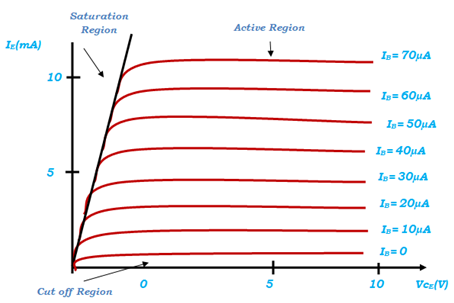
\includegraphics[width=1\columnwidth]{images/trans.png}
        \caption{Typical NPN output characterstics highlighting the sataration and active regions of the transistor}
        \label{th:2}
    \end{figure}
    \begin{figure}[h]
        \centering
        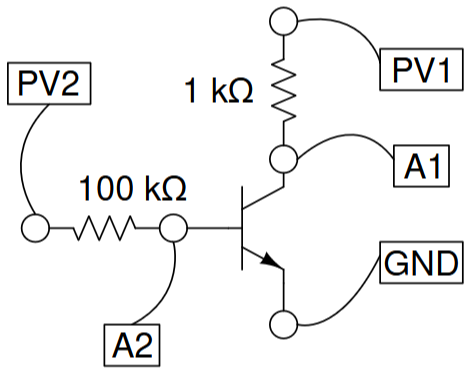
\includegraphics[width=0.7\columnwidth]{images/trans2.png}
        \caption{Circuit diagram for observing the output characteristics of an NPN transistor in CE mode}
        \label{th:2.5}
    \end{figure}
\subsection{Astable multivibrator}
    A Multivibrator is a circuit that oscillates between a ``HIGH" and ``LOW" state, typically with a $50\%$ duty cycle, meaning it has equal ``ON" and ``OFF" times. In sequential logic circuits, the state change may occur on the rising edge, falling edge, or both of the clock signal. On the other hand, stable pulse generation circuits do not have stable states, but rather continuously switch between two states, resulting in a train of square wave pulses at a fixed frequency. These concepts are important in understanding the behavior of multivibrators and pulse generation circuits, and play a significant role in digital electronics and circuit design.
    
    The IC 555 is a popular integrated circuit with 23 transistors, two diodes, and 16 resistors, offering stability and affordability for timer and multivibrator applications. It can operate in mono/bi-stable or astable mode depending on external connections, generating single pulses or continuous pulse trains. Its versatility and characteristics make it widely used in modern electronics.

    \begin{figure}[h]
        \centering
        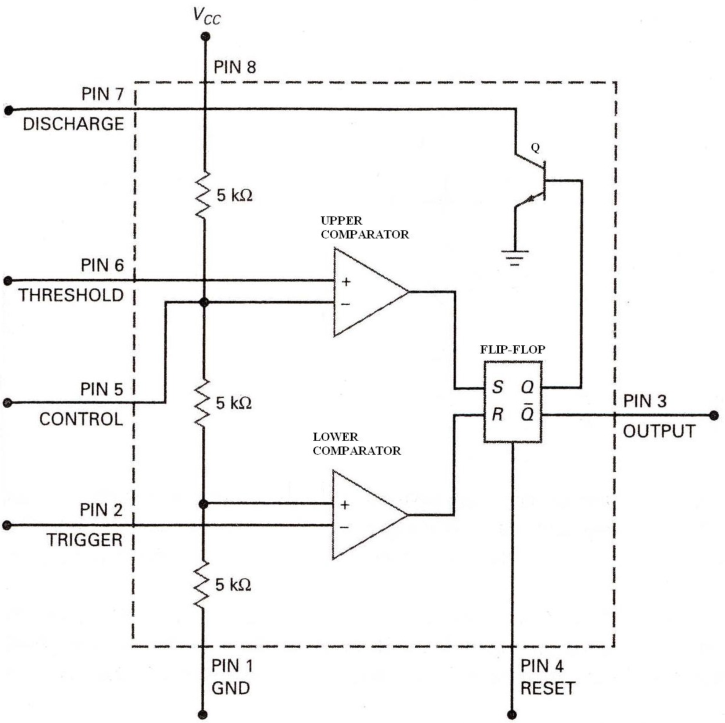
\includegraphics[width=1\columnwidth]{images/555a.png}
        \caption{Functional block diagram of IC 555}
        \label{th:3}
    \end{figure}

    These circuits exhibit instability in any state and trigger output changes after specific time periods. As a result, they generate continuous square/rectangular waveforms with characteristics determined by the values of external resistors and capacitors.

    The circuit diagrams in \hyperref[th:4]{Figure 4} and \hyperref[th:5]{Figure 5} depict the design of astable multivibrator using IC 555, with typical component values. The astable function is achieved by charging or discharging a capacitor through resistors connected to either $V_{cc}$ or GND. The switching between charging and discharging modes is controlled by a resistor divider ($R_A-R_B$), two comparators, and an RS flip-flop within the IC 555. The upper and lower comparators generate positive pulses when the voltage across the capacitor ($V_C$) exceeds $\frac{2}{3}V_{cc}$ or falls below $\frac{1}{3}V_{cc}$, respectively. These positive pulses then set or reset the Q output.

    The astable multivibrator generates a continuous square or rectangular waveform with a duty cycle of $50\%$ or more. The charging and discharging of the capacitor is controlled by the resistors and capacitors connected to the IC 555, which determine the frequency and duty cycle of the output waveform. The resistor values of R1 and R2, along with the capacitor value, determine the frequency of the output waveform, while the resistor values of R1 and R3 determine the duty cycle. By adjusting these resistor and capacitor values, the frequency and duty cycle of the output waveform can be varied to suit the desired application.\\

    \begin{itemize}
        \item The time for charging $C$ from $\frac{1}{3}$ to $\frac{2}{3}$ $V_{cc}$

        (i.e, ON Time $= 0.693 (R_A + R_B)\cdot C$)

        \item The time for discharging $C$ from $\frac{2}{3}$ to $\frac{1}{3}$ $V_{cc}$,
    
        (i.e., OFF Time $= 0.693 R_B\cdot C$)\\
    \end{itemize}

    To get the total oscillation period, adding the two:

        \begin{equation}
        \begin{split}
            T_{osc}& = 0.693(R_A+R_B)C + 0.693(R_B)C \\
            & =0.693 \cdot (R_A + 2\cdot R_B) \cdot C
        \end{split}
        \label{eq:1}
    \end{equation}

    \begin{equation}
        f_{osc} = \frac{1}{T_{osc}} = \frac{1.44}{(R_A + 2R_B)\times C}
        \label{eq:2}
    \end{equation}

    \begin{equation}
        Duty-cycle = \frac{R_A+R_B}{R_A} + 2\times R_B
        \label{eq:3}
    \end{equation}

    \begin{figure}[H]
        \centering
        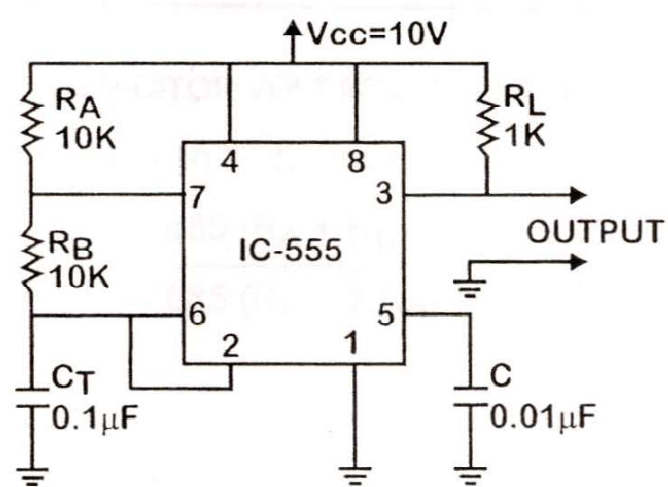
\includegraphics[width=0.8\columnwidth]{images/ast.png}
        \caption{Astable multivibrator circuit with duty cycle less than $50\%$}
        \label{th:4}
    \end{figure}

    \begin{figure}[H]
        \centering
        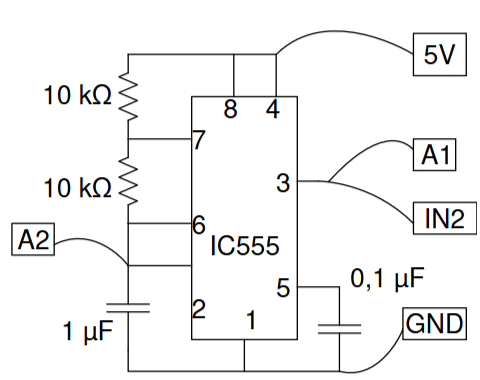
\includegraphics[width=0.7\columnwidth]{images/th5555.png}
        \caption{Astable multivibrator circuit with the SEELab circuit pins highlighted}
        \label{th:5}
    \end{figure}
\subsection{EM induction}

    Faraday's law of EM induction states that anytime the flux connected with a coil changes, an emf is induced in the coil; the direction is determined by Lenz's law and is proportional to the rate of change in flux linkage. Thus, the coil develops an eddy current as a result of this emf. Moving a magnet back and forth across a coil can alter the flux flowing through it. Here, we talk about the scenario when the coil is fixed and the magnet is lowered through it. Unless there is some additional mechanism, air resistance and gravity forces will cause the magnet's velocity to vary. If we drop the magnet vertically along the z-direction keeping the coil at the origin,
    
\begin{figure}[h]
    \centering
    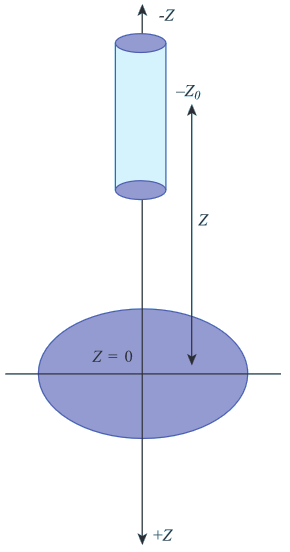
\includegraphics[width=0.5\columnwidth]{images/fall.png}
    \caption{A schematic representation of a magnet falling vertically through a coil.}
    \label{th:7.5}
\end{figure}

    \begin{align*}
        z&=-z_0+ 0.5gt^2\\v&=gt
    \end{align*}

    where $z_0$ is the initial position of the magnet. Here g is the acceleration of the magnet. On passing through the coil, $g$ decreases due to eddy current damping. Eddy current damping is responsible for the time delay in magnets falling through a long conductor. If the coil is short, we can neglect this. So the emf will be:

    \begin{align*}
        emf&=-N\frac{d\phi}{dt}\\&=-N\frac{d(BA)}{dt}
    \end{align*}


    The coil's induced voltage can be expressed as $V = -NAB\sin(\theta)$, where $A$ is the coil's area, $N$ is the number of turns of the coil, and $B$ is the magnetic field produced by the small cylindrical bar magnet at the coil's center. The magnet, with a dipole moment $m$, can be considered as a current-carrying loop with $n$ turns if its length is small.

    \begin{align*}m = n I A = n I\pi R^2\end{align*}

    where R is the radius of the cylindrical magnet. We know that the field along the axis of the circular coil at distance x is given by:

    \begin{align*}B=\frac{\mu_o m}{2\pi}(R^2+x^2)^{-3/2}\end{align*}

    thus emf is given by:

    \begin{align*}emf=\frac{3\mu_o m}{2\pi}NA(R^2+x^2)^{-5/2}xv\end{align*}

    where $v$ is the velocity of the magnet, thus for non-constant velocity emf is given by,

    \begin{equation}
        \begin{split}
            emf=\frac{3\mu_o m}{2\pi}&NA(-z_0+ 0.5gt^2)gt\\
            &\times(R^2+(-z_0+ 0.5gt^2)^2)^{-5/2}
        \end{split}
        \label{eq:4}
    \end{equation}

    \begin{figure}[h]
        \centering
        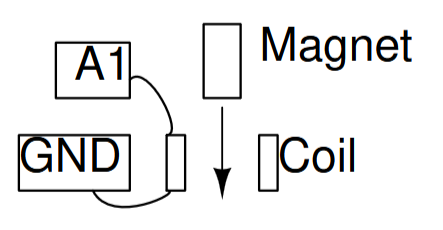
\includegraphics[width=0.5\columnwidth]{images/induc.png}
        \caption{Circuit diagram for EM induction}
        \label{th:6.5}
    \end{figure}

\subsection{Determination of acceleration due to gravity using Rod pendulum}
Period of oscillations of a pendulum depends on it’s length and the value of gravity. Period of oscillation
of a uniform rod about one end is given by \begin{align}T = 2\pi\sqrt{\frac{2l}{3g}}\end{align}where $l$ is the length and $g$ is the acceleration due to gravity.

In this experiment, we measure the period of oscillations of a rod pendulum using a photo-transisor and LED arrangement.
The pendulum (T-shaped, a knife edge attached to a 6mm diameter rod) is made to swing between an LED
and photo-transistor, connected to expEYES. The LED and photo-transistor are mounted on a U-shaped
bracket as shown in Fig. \ref{th:7}.

\begin{figure}[h]
    \centering
    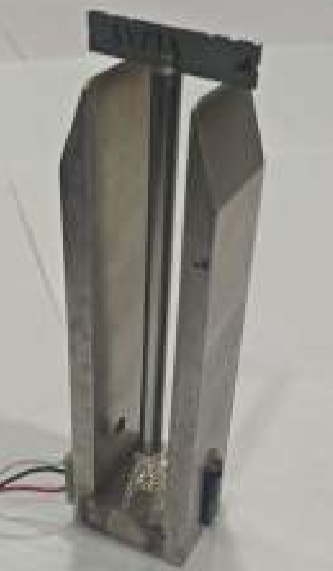
\includegraphics[width=0.4\columnwidth]{images/knifee.png}
    \caption{Rod pendulum, photo-transisor and LED arrangement}
    \label{th:7}
\end{figure}
\begin{figure}[H]
    \centering
    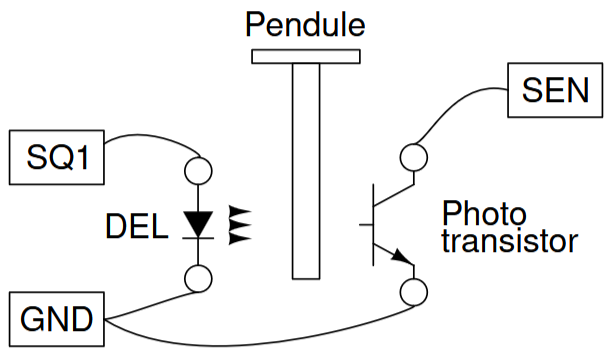
\includegraphics[width=1\columnwidth]{images/pend.png}
    \caption{Circuit diagram for the determination of $g$}
    \label{th:6}
\end{figure}

\subsection{Sound Beats produced by Two Sources with Nearly Equal Frequencies}
Beats are produced when two sinusoidal sound waves of equal amplitude and very nearly equal frequencies mix. When two sound waves of nearly equal frequencies travel in the same direction, at a given point due to their superposition, the intensity alternatively increases and decreases periodically. This periodic waxing and winging of sound at a given position are called beats. 

\begin{align*}
    \begin{split}
        \cos(2\pi f_1t) + \cos(2\pi f_2t) &=\\ 2 \cos& \left(2\pi\frac{f_1+f_2}{2}t\right) \cos \left(2\pi\frac{f_1-f_2}{2}t\right)
    \end{split}
\end{align*}

The second cosine term in the above equationi acts as an envelope for the first cosine series with a reduced frequency of $f_b = f_1-f_2$. This is what we percieve as sound beats.

\begin{figure}[h]
    \centering
    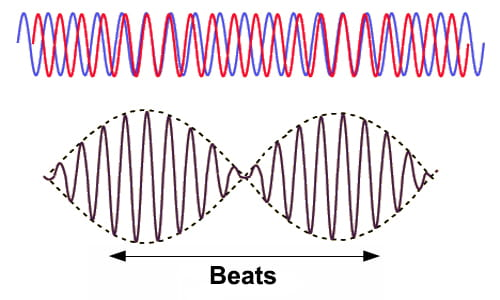
\includegraphics[width=1\columnwidth]{images/Beats.jpg}
    \caption{Two waveforms of nearly equal frequency (above) in superposition, creates the below waveform with an overall envelope}
    \label{th:8}
\end{figure}
\begin{figure}[h]
    \centering
    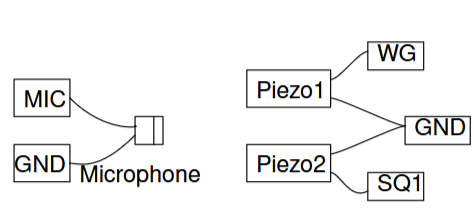
\includegraphics[width=1\columnwidth]{images/beats2.png}
    \caption{Circuit Diagram for observing sound beats}
    \label{th:9}
\end{figure}
% ======================================================================================
\section{Experimental Setup}

\subsection*{Apparatus}

\begin{enumerate}
    \item SEELab 3 Module
    \item EXPEYES17 SEELab3 software
    \item NPN transistor
    \item IC 555 timer
    \item Coil (with number of turns = 5000)
    \item Small magnet (which fits through the coil)
    \item A Rod Pendulum (T-shaped, with a knife
    edge attached to a 6mm diameter rod)
    \item Phototransistor 
    \item Piezo buzzers
    \item Microphone
    \item Capacitors
    \item Resistors
    \item Connecting Wires
    \item Power Supply
\end{enumerate}